% The following choice requires a coordinated choice when PRINTING the report:
%\documentclass[oneside,12pt]{report}  % Use this for one-sided copying (print with printer's normal
%  single-sided option
\documentclass[twoside,12pt,openright]{report}  % You can use this for a slim final printed copy (print with 
%  printer's double-sided option)

% the dimensions of the page
\textheight=9.25in \topmargin=-0.5in   %See note in Chapter 8 of Sample Report about "Page scaling" option in Adobe
\textwidth=6.0in
\oddsidemargin=0.3in
\evensidemargin=0.3in  % Needed to balance even and odd pages in twoside print copy

% Useful packages
\usepackage{amsmath}
\usepackage{amsfonts}
%% In the following, the assumption is that your graphics are in encapsulated postscript (eps).  If not,
%% you may need to use some other method for incorporating graphics into your pdf of the final report.
%  Use the next package for typesetting directly to dvi or postcript (used primarily for the PCTeX typesetter, 
%  see the following alternatives).
\usepackage[dvips]{graphicx} 
% Use the next two packages together for typesetting directly to pdf (this works for pdfLaTeX and may work 
% for others---not yet tested for all---please report your experience).
%\usepackage[pdftex]{graphicx}
%\usepackage{epstopdf}
%%

\usepackage{doc}
% Following sets up logic and formatting for conditional twoside copying
\usepackage{ifthen, color, fancyvrb}
\usepackage{nextpage}\pagestyle{plain}
\newcommand\myclearpage{\cleartooddpage
  [\thispagestyle{empty}]
  }

%  Set font size for captions
\usepackage[skip=4pt,font=footnotesize]{caption}


\DeclareGraphicsExtensions{ps,eps}
\usepackage{excludeonly}

\usepackage{url}
\usepackage{multirow}
\usepackage[super]{nth}
% If some words are being hyphenated incorrectly, they can be
% given in a list to the \hyphenation command as below.
\hyphenation{ap-pen-dix wer-ther-i-an}

% Theorem-like command definitions:
\newtheorem{theorem}{Theorem}[chapter]
\newtheorem{lemma}{Lemma}[chapter]
\newtheorem{definition}{Definition}  % Note, this italicizes everything

% Print the chapter and sections in the toc
\setcounter{tocdepth}{1}

% Specify which files to typeset for this run (note that overall pagination is preserved)
%\includeonly{chapter1, chapter2}

% Specify which files NOT to typeset for this run (note that overall pagination is preserved)
%\excludeonly{}

% Groundwork for allowing double-sided copying with blank versos
\def\prefacesection#1{
\chapter*{#1}
\addcontentsline{toc}{chapter}{#1}
}

\begin{document}

% Footnote references are symbolized in the front matter, but see below for restoration of numbered footnotes in the body.
\def\thefootnote{\fnsymbol{footnote}}

% The title page is in its own file, ``titlepage.tex''.
% It needs to be edited to reflect information specific
% to your project. 
% don't display the page number
\thispagestyle{empty}

% The numbers below controls the amount of space between the following sections
\def\shiftdowna{0.32in}  % Adjust for balance
\def\shiftdownb{0.22in}  % Adjust for balance

% Set up the boiler plate at the top of the page

\begin{center}
\textbf{{\large Summer Research Program in Industrial \\ and Applied Mathematics}}\\

\vspace \shiftdowna
%\includegraphics[width=0.4\textwidth]{ipam.eps}\\

\begin{figure}[h]
  \centering
  \begin{minipage}[b]{0.4\textwidth}
    \centering
    
\includegraphics[width=3cm]{Graphics/HKUST_logo.jpg}
      \end{minipage}
 % \hfill
  \begin{minipage}[b]{0.4\textwidth}
    \centering
    
\includegraphics[width=6cm]{Graphics/snu_logo.jpg}
      \end{minipage}
\end{figure}

% SPONSOR
\vspace \shiftdowna
\underline {Sponsor}\\ 
\vspace{5pt}
$\langle \textbf{{\large Tencent}} \rangle$ \\
\vspace \shiftdowna
\textbf{Final Report}

% TITLE
\vspace \shiftdowna
$\langle \textbf{{\Large Sketch to Image Generation}}\rangle$

% Note the convention used here:  email addresses and urls are typeset in teletype font, colleges are set in italics.

% STUDENTSI
\vspace{0.35in}
\underline {Student Members}\\
\vspace{5pt}
$\langle \text{Seon Gyu PARK}\rangle$ (Project Manager), $\langle \text{\emph{SNU}}\rangle$,\\ 
\vspace{3pt}
$\langle \text{\texttt{SunQ0313@gmail.com}} \rangle$\\
\vspace{5pt}
$\langle \text{Chun Wai WONG}\rangle$, $\langle \text{\emph{HKUST}} \rangle$ \\
\vspace{3pt}
$\langle \text{Fuzhe LI}\rangle$, $\langle \text{\emph{HKUST}} \rangle$ \\
\vspace{3pt}


% ACADEMIC MENTORS
\vspace \shiftdownb
\underline {Academic Mentor} \\
\vspace{5pt}
$\langle \text{Dr. Ningchen YING}\rangle$, $\langle \text{\texttt{mancying@ust.hk}} \rangle$

% SPONSORS
\vspace \shiftdownb
\underline {Sponsoring Mentors}\\
\vspace{5pt}
$\langle \text{Prof. Yu-Wing TAI}\rangle$, $\langle \text{\texttt{yuwingtai@tencent.com}} \rangle$\\
\vspace{3pt}


% CONSTULANTS (comment out this text if there are no consultants)
\vspace \shiftdownb
\underline {Consultants}\\
\vspace{5pt}
$\langle \text{Name}\rangle$\\
\vspace{3pt}
$\langle \text{Name}\rangle$

% DATE
\vspace \shiftdowna
$\langle \text{Date: $7^{\textnormal{th}}$ August 2018}\rangle$ 

\end{center}

%\vfill  %Fill page to force following note to bottom
%\footnoterule
%\noindent \small{This project was jointly supported by HKUST and SNU.} 
 


% Begin ABSTRACT
\ifthenelse{\boolean{@twoside}}{\myclearpage}{}
\prefacesection{Abstract}
% don't display the page number
%\thispagestyle{empty}

This sample report serves two purposes.
First, it introduces the RIPS ``house style''---preferences for how copy is set and laid out on a page.%%
\footnote{
R. M. Ritter, {\em New Hart's Rules:  The Handbook of Style for Writers and Editors}, Oxford University Press, 2005.
}
Second, by comparing this document with the {\LaTeX} source, it illustrates the effects of {\LaTeX} code on the resulting typeset.%
\footnote{
Location of the source code is provided in Appendix \ref{App:SourceLocation}.
}

\vspace{24pt}
(The Abstract should succinctly summarize the purpose and results of the RIPS project. 
Usually, it will be one paragraph of no more than half a page to one page in length.
The Abstract is often the last major component to be written, since it is almost impossible to know what to say until you have essentially completed the project.

The Abstract is self-contained.
For example, unfamiliar acronyms should be used sparingly, and if used, should also be spelled out.
References to the literature should be specified completely, not cited for look-up in the Bibliography.)%%
\footnote{
Note that in front matter the footnote reference can be a symbol, but in the body it is usually a number.
}


% Begin ACKNOWLEDGMENTS
%\ifthenelse{\boolean{@twoside}}{\myclearpage}{}
%\prefacesection{Acknowledgments}
%It is appropriate in the Acknowledgments to thank individuals or organizations who made especially noteworthy contributions to your project.
Elsewhere, within the body of the report, you can acknowledge more specific contributions where appropriate.
These are matters of courtesy and professional ethics.
As an example:

\begin{quote}
The RIPS {\LaTeX} report template has been developed by Mike Raugh with advice and assistance from Oleg 
Alexandrov and Shawn Cokus in the early stage of development and general support of IPAM and the System Administration staff.
The first RIPS template was based on an early version of the Math Clinic's report template at 
Harvey Mudd College;
there the original template has been improved and is managed by Claire Connelly, the HMC Math Department's system administrator.  
Claire and her co-authors offer coding advice, a wealth of references, and a note about the origin of the template in their current 
edition, the $\texttt{sample-clinic-report.pdf}$ accessible at $\texttt{ http://www.math.hmc.edu/computing/support/tex/sample-report}$.
Claire copyedited the third edition of Gr\"{a}tzer's \emph{Math into {LaTeX}}, most of which
work seems to have survived into the fourth edition:  \emph{More Math into {LaTeX}} \cite{gratzer}.
\end{quote}

When acknowledging individuals in this section, it is OK to use the names by which you know and speak to them.
Here it is OK to write ``Oleg Alexandrov.''
But you must be formal on the Title page and elsewhere within the report, where it is proper to specify honorifics, e.g., Dr. or Prof.
On the Title page you would write ``Dr. Oleg Alexandrov,''
and likewise within the body of the report if you were acknowledging him for a specific contribution, 
Claire Connelly uses no honorific, so you would use just her name on the title page.
When in doubt, check the person's business card or follow usage on the person's web page.

\vspace{8pt}
As a result of suggestions from users, this Sample Report and its source are under continual improvement.
Please contact the RIPS program director for your suggestions.
An up-to-date  list of changes is recorded in the "Revisions" folder for the Master Template Folder.
%%



% Table of contents, List of Figures, and List of Tables.
\ifthenelse{\boolean{@twoside}}{\myclearpage}{}
\tableofcontents

\ifthenelse{\boolean{@twoside}}{\myclearpage}{}
\listoffigures

\ifthenelse{\boolean{@twoside}}{\myclearpage}{}
\listoftables

% The report is an extensive document.
% It is convenient to have each chapter of the report in its own file
% rather than throw all work together in a single file.
% Do not run the LaTeX typesetter on each individual chapter; refresh
% your report by running the typesetter on this master file.

% Cancel the previous symbol requirement for footnotes in the front
% matter, and use arabic numerals for footnotes in the body
\renewcommand{\thefootnote}{\arabic{footnote}}
\setcounter{footnote}{0}

% Chapter 1 -- the Introduction
\ifthenelse{\boolean{@twoside}}{\myclearpage}{}
\chapter{Introduction}\label{Ch:Introduction}

\section{Project Goal}

The goal of this project is to build a system that can generate photo-realistic images from rough sketch pictures. 

\section{Related Works}

Sketch-to-Image generation is a sub-problem of Image-to-Image translation where the goal is to 
learn the mapping between distinct domains of image. 
In 2017, Jun-Yan Zhu et al. achieved transforming a horse image into a zebra using Cycle-Consistent Adversarial Networks. However, in the Sketch-to-Image generation, the mapping between photo and sketch always cause loss in dimension of data, resulting in losting the uniqueness of mapping. Our goal is to train a Cycle-Consistent Adversarial Networks to learn a mapping \(G:X \rightarrow Y\) such that the distribution of images from \(G(X)\) indistinguishable from the distribution \(Y\) using an adversial loss. In other word, it can generate high quality photo from a sketch image.\\%%%Can put more detail on the introduction of GAN above %%%Some result we achieved %%%\\


The team would like to thank \emph{Tencent} for the generous sponsorship of this project. 
% Founded in November, 1998, Tencent is a leading provider of Internet value added services in China. Since its establishment, Tencent has maintained steady growth under its user-oriented operating strategies. On \(16^{\textnormal{th}}\) June 2004, Tencent Holdings Limited (SEHK 700) went public on the main board of the Hong Kong Stock Exchange.\\


%%%Something about the Related Work%%% \\

Our code is available at \texttt{https://github.com/SunQpark/SPIA2018\_cycle\_GAN}.




\endinput


% Chapter 2
\ifthenelse{\boolean{@twoside}}{\myclearpage}{}
\chapter{Background}\label{Ch:Background}
\section{Related Models}
There are two main approaches for image generation tasks: generative adversarial nets and variational autoencoder. In this project, only GAN-related methods will be considered and inplemented.
The original GAN proposed by Goodfellow can train a generator to learn the real image distribution by training a discriminator together, which can tell the difference between real images and fake images.

In the field of image translation trained with unpaired image datasets, 3 models, CycleGAN, DiscoGAN, DualGAN are doing the same thing
from high level perspective. They train two generative models to learn the mapping between two image domains by training two discriminators
at each domain together and considering the cycle-consistency loss, which ensures ignorable difference between images and reconstructed images.
\\
In detail, the differences are
CycleGAN uses instance normalization, patchGAN discriminator. To stabilize the training, use least square GAN. Replay buffer
              no random input z no drop out; L1 distance as cycle consistency

DualGAN use generator and discriminator of pix2pix; no random input z but implemented drop out; use wgan;
             L1 distance as cycle consistency

DiscoGAN generator: conv, deconv and leaky relu; discriminator:conv+leaky relu  L2 distance as cycle consistency


\endinput


% Chapter 3
\ifthenelse{\boolean{@twoside}}{\myclearpage}{}
\chapter{Methodology}\label{Ch:Methodology}


\section{Collection and Refinement of Data}
In this section, we will explain about the progresses of collecting and refining data we've gone through. 
Table % TODO: add table about composition of dataset
shows the composition of dataset we used in experiments. 

\subsection{Photograph}

For realistic photographs of human faces, we used Celebrity A~\cite{liu2015faceattributes} which contains more than 200,000 images of celebrity in the world. In addition to having clean images of human faces, this dataset contained `attributes', some additional imformation of images. Though those informations were not used directly as input to our neural networks, they were useful in some progress of preprocessing. We will describe about the details in ~\ref{preprocess}.

\subsection{Sketch}

The main portion of sketch image dataset we used was collected from Google Image search engine. However, the collected images were highly inconsistent, which was undisirable. 
figure %TODO: add figure: bad examples
shows some bad examples of image which were included in the first collection. Thus, these images has gone through preprocessing steps, which will be described in next section~\ref{preprocess}
After preprocessing steps, these images were aligned as fig%TODO: add figure: after preprocess

We also used CUHK(The Chinese University of Hong Kong) face sketch database(CUFS)~\cite{CUHK_faces}, containing about 500 face sketches. 
Although this dataset also provides face photographs paired with the sketch images, we only used the sketch images to train our model to keep it from overfitting to these paired images.

Examples of images in each dataset can be seen in fig.%TODO: add figure: example of images in dataset

\subsection{Preprocess}\label{preprocess}

In this section we deals with the preprocessing steps on face sketches and photos, which were applied separately before the training of model. By experiments of a few weeks, we found this part crucial to the performance of model. 
The first step of data refinement was to detect every faces for each image. By excluding images not containing recognized faces, we could get rid of 20\% of bad examples in sketch database. Then, we applied `facial landmark detection' for the detected faces, in order to get further information concerning the direction of head in the images. We utilized the `dlib' framework ~\cite{dlib} for those two steps.
Next, we rotated the images to have faces aligned vertically using the detected locations of two eyes.
Finally, the images were cropped to have faces in center and 30\% of the width of head margins on both sides. The cropped images have 128 by 128 size in the end of preprocessings. Those steps were applied to both sketch and photo images to make them consistent in any attributes other than it is sketch or photo. 

After some experiments we found that the model was learning to put smile on the generated photo from sketch images even when the original sketch images were not smiling. This seemed to be originated from the fact that images in photograph have smile in most case, while sketch images haven't. Since this was undisired effect, we reduced the ratio of smiling faces in the photograph dataset. This process was done by checking attributes file which Celebrity A dataset provided to see wether given image is smiling or not and using only one images per 20 smiling images.

\section{Model Structure}

As we mentioned earlier, baseline structure mainly used in this project is Cycle-GAN. The Cycle-GAN consists of two GAN models, which learn to translate images from one domain to the other, one direction per each respectively. 


\section{Stabilization of GAN Training}


\section{Evaluation Metric}

`Inception Score'~\cite{improved_tech_GANs}
While there are some of defeats ~\cite{note_on_inception}

\endinput


% Chapter 4
\ifthenelse{\boolean{@twoside}}{\myclearpage}{}
\chapter{Sample figures and tables}\label{Ch:figures}

\section{Figures}

% Note that the label follows the caption.
\begin{figure}[ht]
\begin{center}

\includegraphics[width=0.3\textwidth]{Graphics/ipamlogo.eps}
\end{center}
\caption{A sample \textsc{eps} figure with a caption.}\label{FIGURE:IPAM-logo-eps}
\end{figure} 


\subsubsection{Formats accepted by {\LaTeX}}
This version of the  RIPS {\LaTeX } template can be used to produce a pdf of your report using several different typesetters, including \texttt{pcTeX} and other options available on the IPAM network.
All of these will accept figures in the encapsulated postscript (\textsc{eps}) format providing you incorporate the appropriate \emph{packages} in the \emph{preamble} of your {\LaTeX] code.%%
\footnote{
The RIPS reports template devotes a section of the preamble to a method for ensuring that your chosen typesetter will be able to utilize eps files. 
This is one of several options for affecting formats that you will find explained by comments in the preamble.
For a good source for general information on incorporating graphics in {\LaTeX}, see
\texttt{http://amath.colorado.edu/documentation/LaTeX/reference/figures.html}.
}%% 
The LaTeX code for Figure \ref{FIGURE:IPAM-logo-eps} shows how to emplace, label and reference it.
You may have to convert the format for your figure.
But beware, incorporating graphics in {\LaTeX} can be quirky and require special attention and work-arounds.%%
\footnote{There is a simple way to make format conversions that works in some cases.
Click on the file in its current format, then when the graphic appears on your screen use ``save as'' to write the graphic in a format you select from the given options.
See Chapter 7 for more suggestions.}

\subsubsection{Creating figures with {\textsc{Matlab}}}
Here's a sample code, describing how to create a figure in \textsc{Matlab} and export it as \textsc{eps}.

\begin{verbatim}
%% Shows how to make a MATLAB figure

%% create a vector of N points between a and b
a=-1.2; b = -a; N = 100; X=linspace(a, b, N);

Y = X.^3 - X; % a function of X

figure(1); clf; % pop up a figure, clean it

H = axes; set(H, 'fontsize', 20); % set the font

plot(X, Y, 'color', 'blue', 'linewidth', 2); % plot

axis([a, b, -0.6, 0.6]); % the viewable box

saveas(gcf, 'MyPicture.eps', 'psc2'); % save the picture in color
\end{verbatim}

\begin{figure}[h]
\begin{center}
\includegraphics[clip, width=0.4\textwidth]{Graphics/MatlabPicture.eps}
\caption[A sample figure created as an \texttt{eps} file by \textsc{Matlab}]{A sample figure created as an \texttt{eps} file by \textsc{Matlab}.
To see an example of quirky treatment, compare this figure when you typeset the report template with \textsc{PCTeX} and pdf{\LaTeX}.}\label{FIGURE:fromMatlab}
\end{center}
\end{figure}

The source code for Figure \ref{FIGURE:fromInkScape} is available in the sample RIPS report directory. 
The {\LaTeX}code for incorporating this figure in the report template is:

\vspace{8pt}
\begin{quote} 
{\tt $\backslash$begin\{figure\}[h]\\
{\tt $\backslash$begin\{center\}} \\
{\tt $\backslash$includegraphics[clip, width=0.4$\backslash$textwidth]{Graphics/MatlabPicture.eps}} \\
{\tt $\backslash$caption\{A sample figure created with $\backslash$textsc\{Matlab\}.\}}$\backslash$label{<name of label}}  \\
{\tt $\backslash$end\{center\}} \\
{\tt $\backslash$end\{figure\}}
\end{quote}

Beware: your label identifier should always follow the caption statement.
You can place it higher up without crashing the {\LaTeX} compiler, but doing so can result in an erroneous enumeration for the label in your text.

\subsubsection{Software for drawing diagrams}

There exist many programs for drawing figures and diagrams.
If you have a preferred system, please let the RIPS director know about it.
Maybe it should be referenced here.
The following two were recommended by Academic Mentors:

\textsc{PSTricks} is a powerful system for designing and incorporating fine mathematical graphics into {\TeX} and {\LaTeX} documents.
Be aware that it works directly with inline code for some {\LaTeX} typesetters but  requires special handling for pdf{\LaTeX}.  
See Figure \ref{FIGURE:fromPSTricks}.


\begin{figure}[h]
\begin{center}
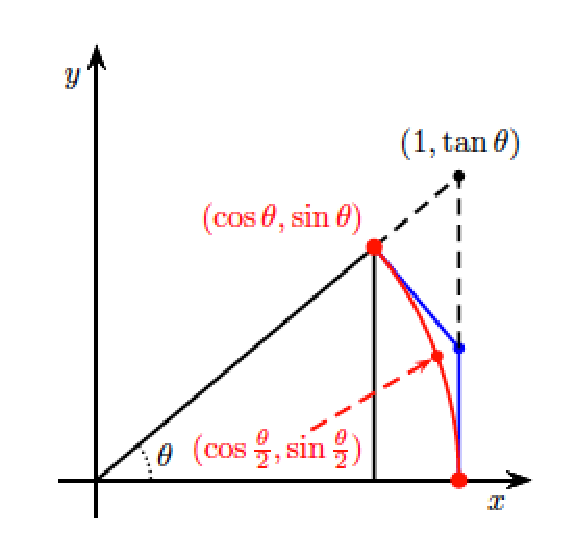
\includegraphics[clip, width=0.4\textwidth]{Graphics/SineTheta5-CS.eps}
\caption[A sample figure created as an \texttt{eps} file by \textsc{Matlab}]{PSTricks code for this figure is in the ``Graphics'' folder for the {\LaTeX} template.
The code was run using Xe{\LaTeX} and the resulting \texttt{pdf} file was converted to an \texttt{eps} file.}\label{FIGURE:fromPSTricks}
\end{center}
\end{figure}


\emph{Inkscape} is free and of high quality;
with this program, you should always keep the figures in Inkscape's native \textsc{svg} format,
and save them as \textsc{eps} only in order to view them in {\LaTeX}.


\begin{figure}[ht]
\label{fig2}
\begin{center}
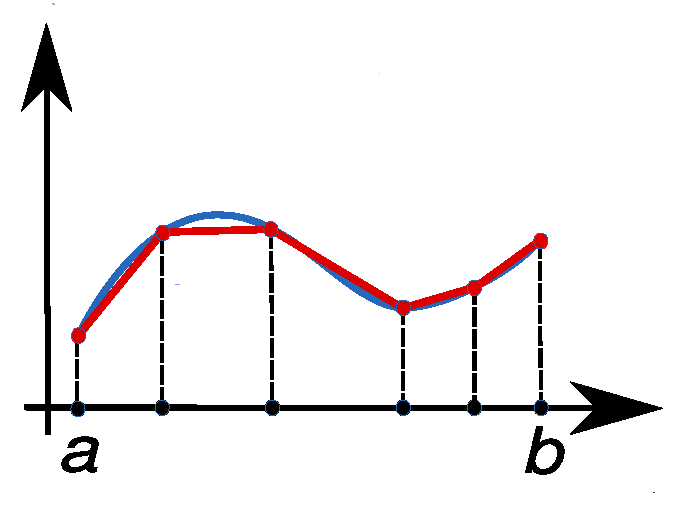
\includegraphics[width=0.4\textwidth]{Graphics/Figure1.eps}
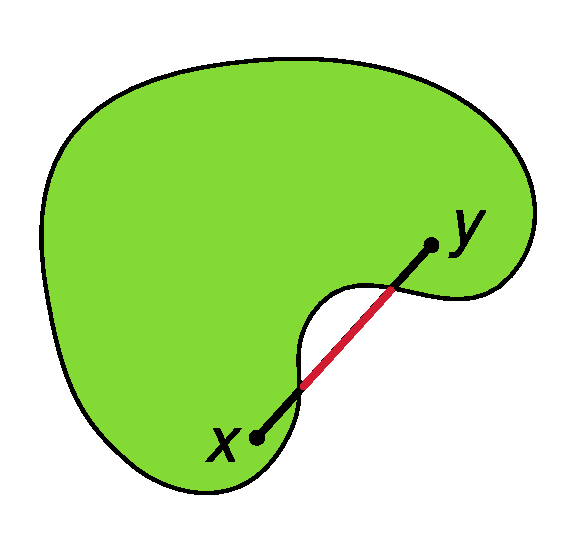
\includegraphics[width=0.309\textwidth]{Graphics/Figure2.eps}
\end{center}
\caption{A couple of figures drawn with Inkscape.}\label{FIGURE:fromInkScape}
\end{figure}

The two adjacent graphics in Figure \ref{FIGURE:fromInkScape} were created with Inkscape and exported to \textsc{eps}.
The figures in the original \textsc{svg} format are available in the report directory.
Note that the convention for punctuating a figure caption or table caption is pretty loose.
If an initial phrase is followed by a complete sentence, the phrase as well as any complete sentence should be ended with a period.
For consistency, it is \textsc{ok} to end all captions with a period even if a caption is just a phrase, as are all three captions illustrated here.

\section{Tables}

\noindent The next example is a simple table: Table \ref{TABLE:Simple}.
The {\LaTeX} code for it is presented after the table. 

% Note that the label follows the caption.
\begin{table}[h]
\begin{center}
  \begin{tabular}{|lcc|}
    \hline
    Date & High & Low\\ \hline
    1-Jul & 40 & 12\\
    2-Jul & 37 & 14\\
    3-Jul & 35 & 20\\ \hline
  \end{tabular}
\end{center}
\caption{A simple table showing fictional data.}\label{TABLE:Simple}
\end{table}

Look at the following source code for Table \ref{TABLE:Simple}, and note particularly how it is labeled.
The references to it in the two preceding sentencs were created by incorporating the label in the {\LaTeX} code 
(``\verb+Table \ref{TABLE:Simple}+'') used for creating this chapter.
Tables are labeled and referenced in a way similar to figures.

\begin{verbatim}
% Note that the label follows the caption.
\begin{table}[h]
\begin{center}
  \begin{tabular}{|lcc|}
    \hline
    Date & High & Low\\ \hline
    1-Jul & 40 & 12\\
    2-Jul & 37 & 14\\
    3-Jul & 35 & 20\\ \hline
  \end{tabular}
\end{center}
\caption{A sample table showing fictional data.}\label{TABLE:Simple}
\end{table}
\end{verbatim}

The next example, Table \ref{TABLE:SplitText}, illustrates a table in which column widths are specified by parameters in order to force long text to be spread over more than one line: 

\begin{table}[h]
\begin{center}
\begin{tabular}{|p{1in}|p{2in}|} \hline
Betty & Betty has a story to tell. \\ \hline
Bob   & Bob has a longer story to tell. \\ \hline
Bill  & Bill has a very much longer and far more dramatic story to tell. \\ \hline
\end{tabular}
\caption{A sample table with split lines of text.}\label{TABLE:SplitText}
\end{center}
\end{table}

\noindent Here's the code for Table \ref{TABLE:SplitText}:

\begin{verbatim}
\begin{table}[h]
\begin{center}
\begin{tabular}{|p{1in}|p{2in}|} \hline
Betty & Betty has a story to tell. \\ \hline
Bob   & Bob has a longer story to tell. \\ \hline
Bill  & Bill has a very much longer and far more dramatic story to tell. \\ \hline
\end{tabular}
\caption{A sample table with split lines of text.}\label{TABLE:SplitText}
\end{center}
\end{table}
\end{verbatim}

\subsubsection{Style tips about figures and tables}
You should always make sure that your figures are easy to see, so for example, make sure that any curves are not too thin or text is not too small.
And don't forget to include axis labels with units specified.

Your figures should look good both in color and as black-and-white, since for presentations you will most likely want figures in color, while in a printed report all the figures will usually be printed in black-and-white (and then, what looks very clear and pretty on your screen may appear as a dark region on paper).

Good captions greatly improve the usefulness of figures and tables.

But no matter how well a caption describes a figure or table, you should always reference it and explain it in your text.
You may feel you are being redundant, but your readers won't think so:
a picture with a good description is worth a thousand words, and a picture without a description in the text is left dangling.

\section{Picking nits}
Notice that in this sample report, all of the captions for figures and tables are placed below the object, and their labels end with a numbered identifier---e.g., Figure 4.1, Table 4.2---terminated with a colon (``:'') inserted automatically by the {\LaTeX} compiler. 
\emph{The Chicago Manual of Style} specifies the use of a period (``.'') to follow the figure number and a blank space to follow the table number, and \emph{New Hart's Rules} follows both figure and table numbers with a blank space.  
Moreover, \emph{New Hart's Rules} places table captions above the table, rather than beneath.
But here we bow to usage in {Gr\"{a}tzer's} \emph{More Math Into {\LaTeX}}(See Bibliography for references).
In such minutiae it's your choice, but remember, consistency (perhaps a hobgoblin of lesser minds but certainly a ruling passion in typography) is standard practice. 


Another place to be on guard is in referencing, e.g., sections, equations, and lemmas.
Do you capitalize or leave it in lower case: Chapter 1 or chapter 1, Theorem 1 or theorem 1, Lemma 1 or lemma 1?
Of course at sentence heads you have no choice but to capitalize.
When you refer to a figure or a table, you may write, for example, ``Fig. 1'', ``Figure 1'', with or without an initial capital, and write ``Table 1'' or ``table 1''.
Recommended usage for this report is to use proper nouns: whether abreviated or spelled out in full, capitalize the labels.
It's up to you, but be consistent.

You'll think of other things as you go along.
Just consider how it looks on the page, and {\it be consistent throughout your report}.

\endinput



% Chapter 5
\ifthenelse{\boolean{@twoside}}{\myclearpage}{}
\chapter{Result}\label{Ch:Result}

Figure~\ref{FIG:before_refinement} shows some examples of result before the data refinement steps were applied. The results seems to contain some face-like objects, but the original faces in the sketch images were not properly translated, resulting in weired colorization in the result. The result of photograph to sketch translation also shows severe artifacts due to the mismatch of locations of faces between datasets.

\begin{figure}[ht]
    \begin{center}
    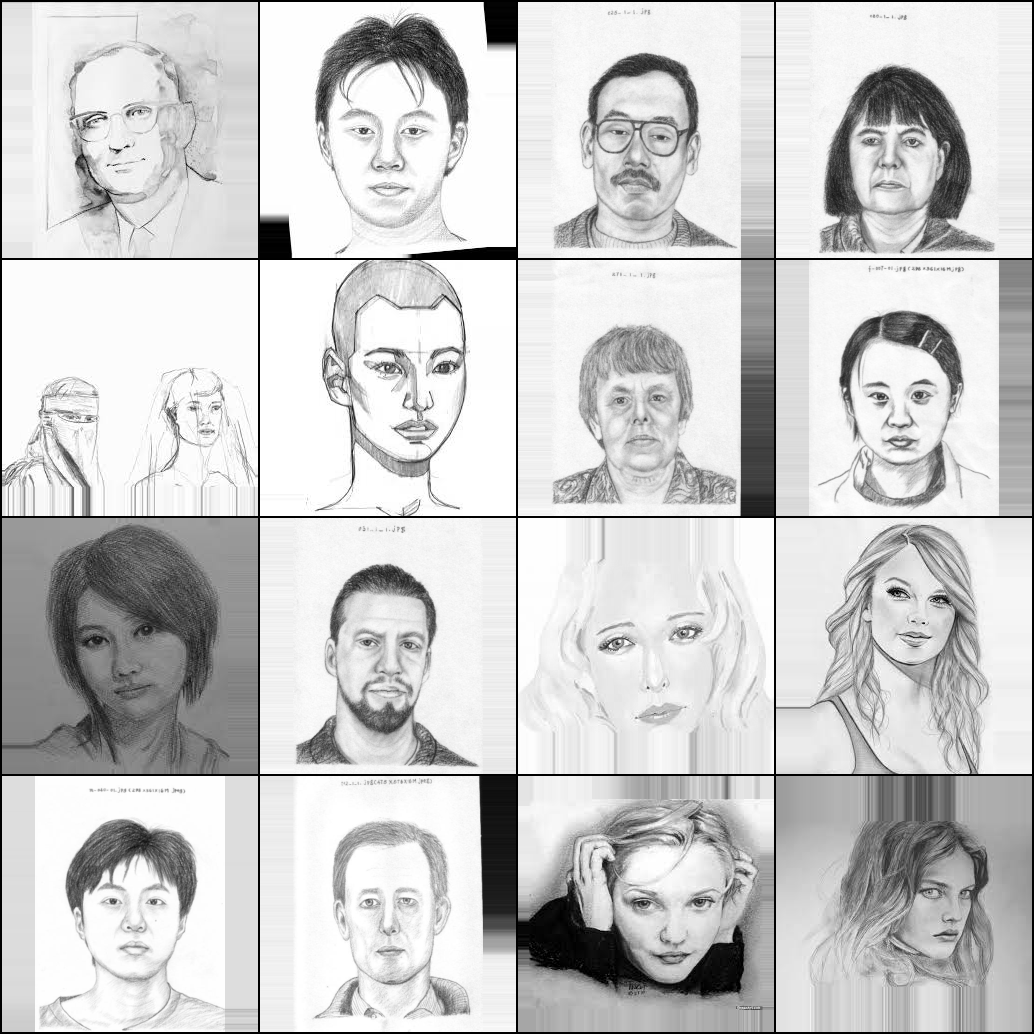
\includegraphics[scale=0.16]{Graphics/ske2pic_origin_before_clean.png}
    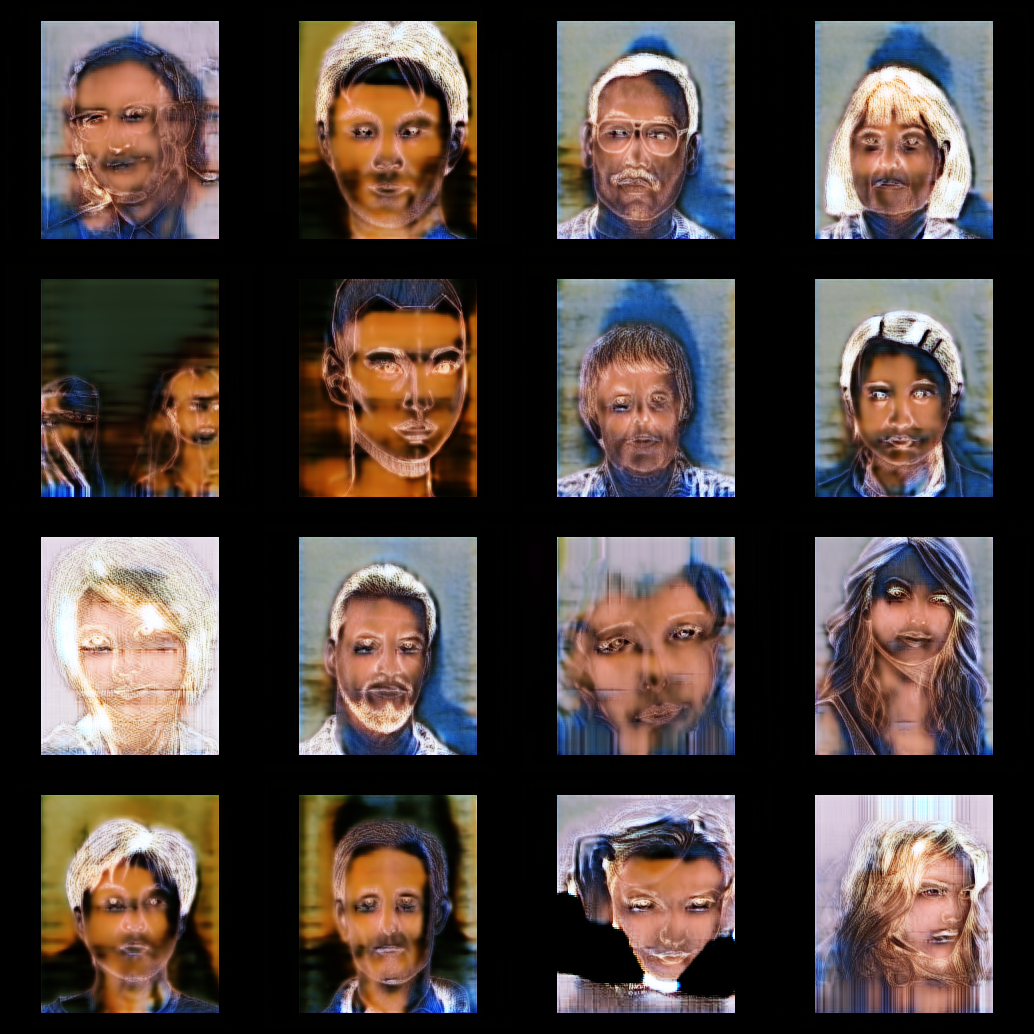
\includegraphics[scale=0.16]{Graphics/ske2pic_result_before_clean.png}

    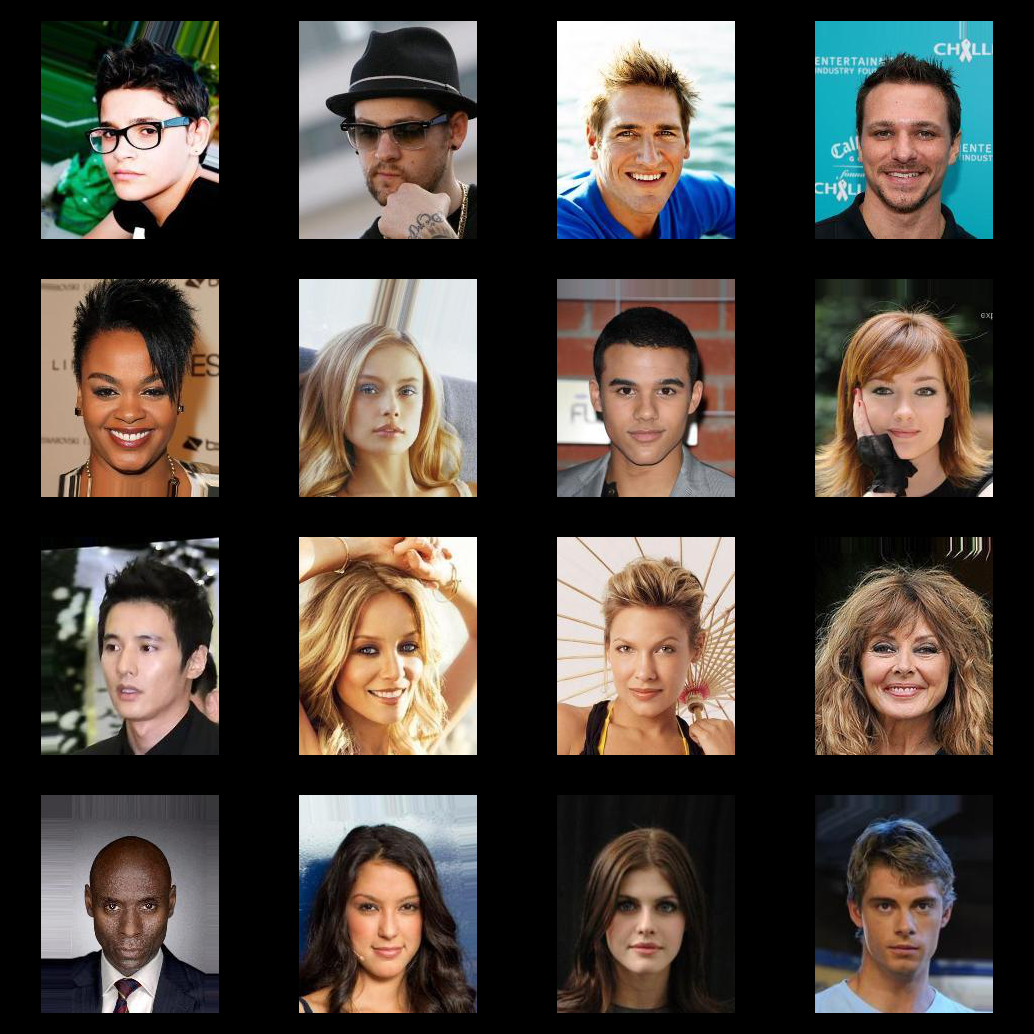
\includegraphics[scale=0.16]{Graphics/pic2ske_origin_before_clean.png}
    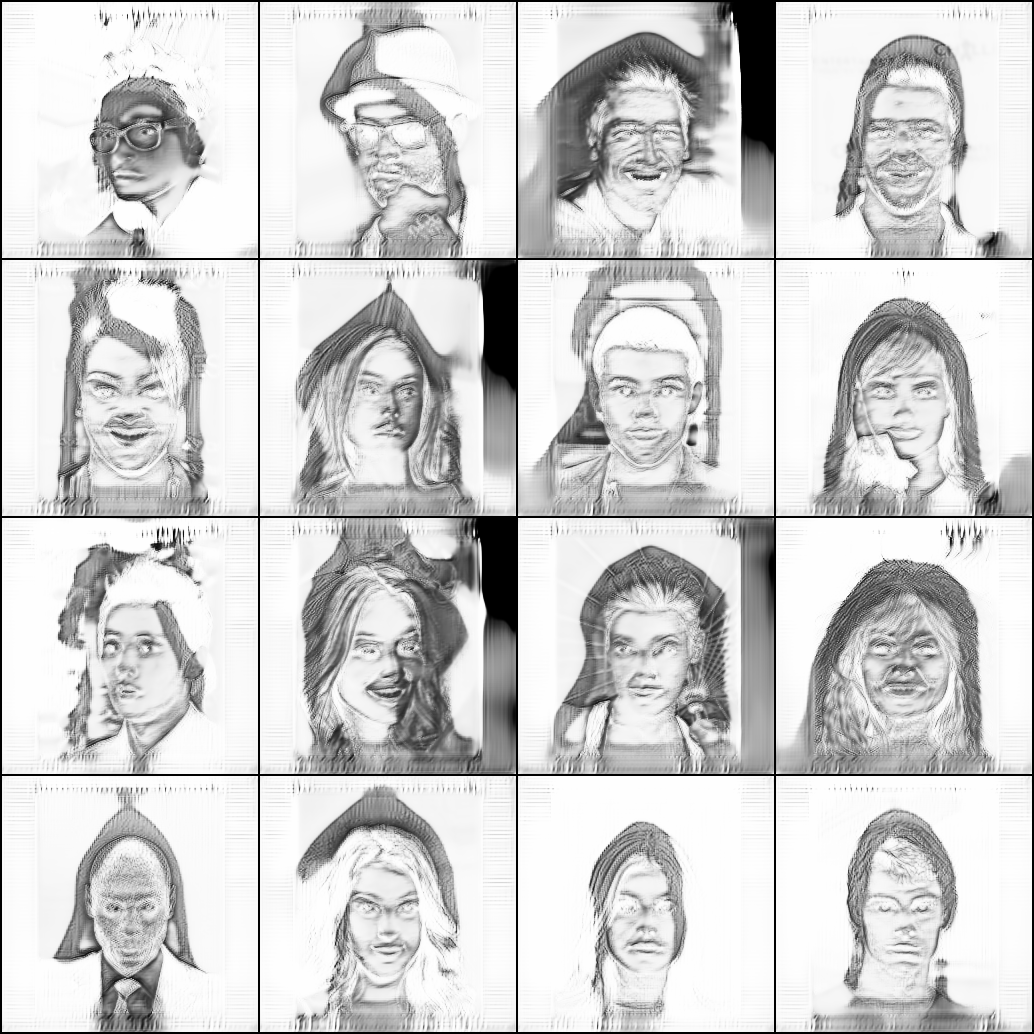
\includegraphics[scale=0.16]{Graphics/pic2ske_result_before_clean.png}
    \end{center}
    \caption{Original input images(left) and result of translations(right) by networks trained before input data is not aligned. Image size is 256 by 256 and model is trained for 64 epochs.}\label{FIG:before_refinement}
\end{figure}

The result seems to be improved considerably with preprocessing steps. Fig~\ref{FIG:smile} shows aligned faces helped the model tell the face and background apart, resulting it to generate better volumes, colors on the paintings. 

\begin{figure}[ht]
    \begin{center}
    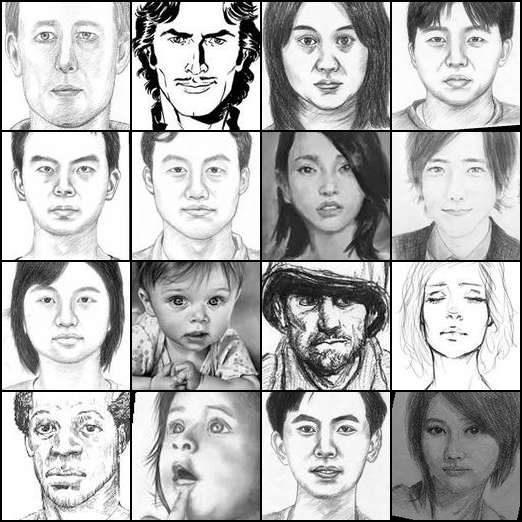
\includegraphics[scale=0.32]{Graphics/smiling_input.png}
    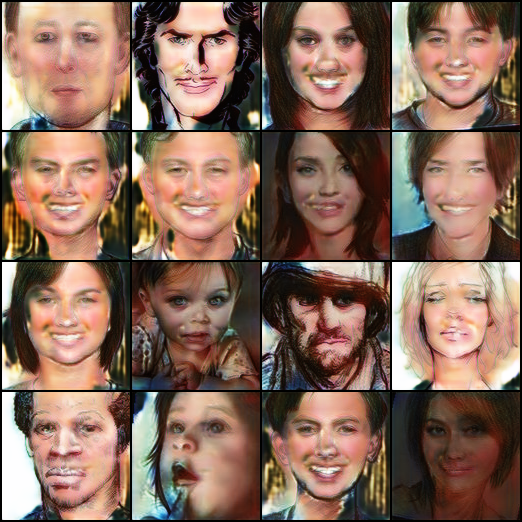
\includegraphics[scale=0.32]{Graphics/smiling_output.png}
    \end{center}
    \caption{Original input images(left) and result of translations(right) by networks trained on datasets after face alignment, but before number of smiling faces was reduced. Image size is 128 by 128 and model is trained for 128 epochs.}\label{FIG:smile}
\end{figure}

However, the results still looks not realistic, mostly due to mistakenly generated smile on the translated images. After some investigation we could find out that is due to the difference of distribution of train data that people smiled much more on the photos rather than on the paintings.
After reducing the ratio of smile in the photograph dataset used as in previous chapter~\ref{Ch:process_data}, we could get following results~\ref{FIG:final}.

\begin{figure}[ht]
    \begin{center}
    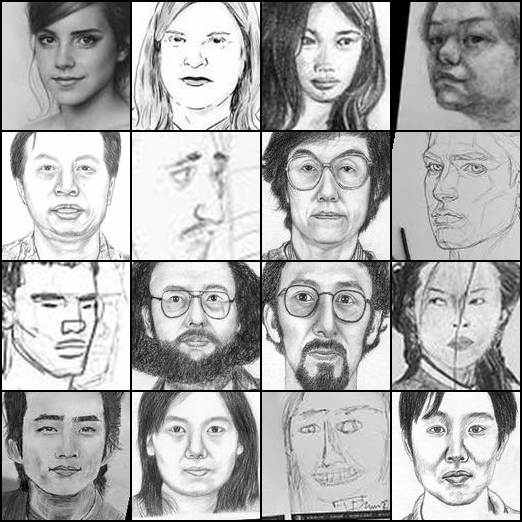
\includegraphics[scale=0.32]{Graphics/ske2pic_origin_final.png}
    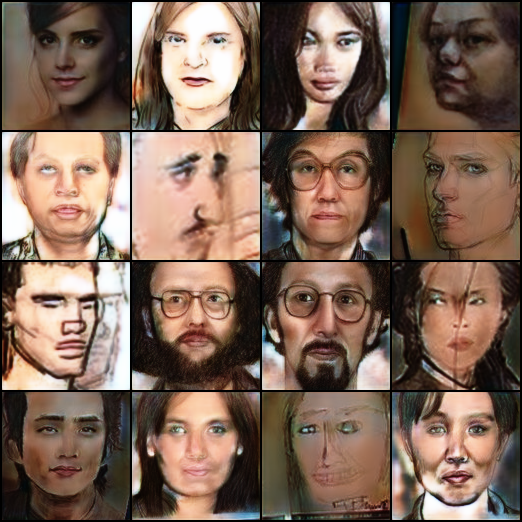
\includegraphics[scale=0.32]{Graphics/ske2pic_result_final.png}

    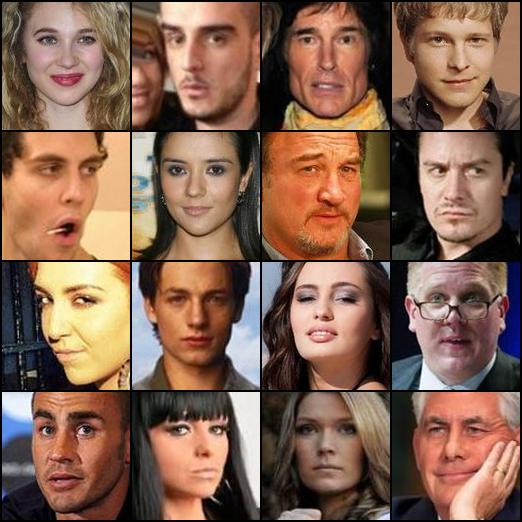
\includegraphics[scale=0.32]{Graphics/pic2ske_origin_final.png}
    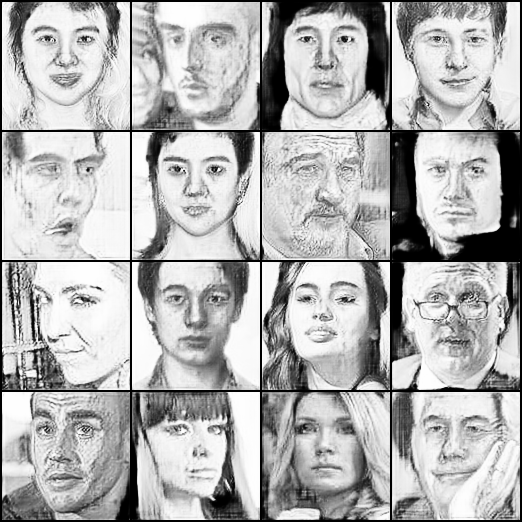
\includegraphics[scale=0.32]{Graphics/pic2ske_result_final.png}
    \end{center}
    \caption{Original input images(left) and result of translations(right) by networks trained on datasets after face alignment and number of smiling faces was reduced. Image size is 128 by 128 and model is trained for 128 epochs.}\label{FIG:final}
\end{figure}

While some of the sketch-to-photo results seems quite realistic(\nth{3} image of \nth{2} column, \nth{2}, \nth{3} of \nth{3}), images generated from low-quality inputs does not seems to be properly translated(\nth{2} image of \nth{2} column, last ones in \nth{3}, \nth{4} column). 
On the other hand, despite the general quality looks fine, some of results(\nth{1}, \nth{2} diagonal positions) resembles average sample images of CUFS datasets rather than contents of input.

% TODO: move to conclusion?
Considering the quantity and quality of sketch images collected from google image search, this amount of dependency on input might be considered acceptible.

\endinput


% Chapter 6
\ifthenelse{\boolean{@twoside}}{\myclearpage}{}
\chapter{Giving credit where credit is due}\label{Ch:GivingCredit}

The point was made in the Acknowledgments section of this Sample Report that it is important to credit others whose work you use---it is a matter of professional ethics and courtesy. 
In addition to acknowledgment of broad assistance or contributions that you put into the Acknowledgments, you may also need to reference more specific contributions elsewhere in your text.
Wherever a distinction is needed, make it clear which part of your work you have borrowed or adapted from others, and provide a reference to the source. 


\endinput


% Chapter 7
%\ifthenelse{\boolean{@twoside}}{\myclearpage}{}
%\chapter{Some extra advice for starting up with {\LaTeX}}\label{Ch:ExtraAdvice}

The following is a small collection of answers to questions RIPS students have asked.

\begin{enumerate}

%%%%
\item {\bf How do I open and modify {\LaTeX} files, as well as view the results?}
%%%%

Several {\LaTeX} typesetters are available on the IPAM network.
The default options are activated by clicking on the  main page for the report template,\\ 

\centerline{\texttt{z-Report-Master-2015.tex}}
\vspace{5pt}

The present version of the template is being maintained using the TeXworks typesetter "pdfLaTeX."
For more information about other options, see the  README file listed among the files used in construction this report.

\hspace{15pt} The template is divided into several chapters, appendixes and other files with functions identifiable by their names coded in {\LaTeX} (files ending in ``.tex'') along with some graphics files coded as Encapsulate Postscript (``.eps'').  
If you modify any one of these source files, you will need to run the typesetter on the main \texttt{z-Report-Master-2015.tex} file.
See Chapter \ref{Ch:References} for tips handling bibliographic references.
And see Appendix \ref{App:SourceLocation} for location of the {\LaTeX} sources relating to this sample report.

%%%%
\item {\bf Should I use a single-sided or double-sided format for my report?}
%%%%

Clearly, double-sided printing saves paper.
But this is not as simple as it seems.
Best to explain this in vocabulary used by publishers: {\em opening}, {\em recto}, and {\em verso}:
An {\em opening} is the pair of pages you see when you open a book at random; the recto is the page on the right-hand side, and the verso is the page on the left-hand side --- or, on a single leaf, recto is the front side and verso is the opposite side.
When you open almost any book at the start of a new chapter, the first page of the chapter will appear on the right-hand page---{\em recto}.
This is true whether or not the left-hand page of the opening---{\em verso}---is blank.
That's the way it should be in your report.
Each major section of your report, not just chapters, should begin on a recto.

\hspace{15pt} Rectos are always odd-numbered.
Very likely, you will not get these results if you submit your single-sided report for double-sided copying on a printer.
There are some {\LaTeX} acrobatics you must specify to make your double-sided report turn out with proper recto-verso pagination, the code for which is built into  \texttt{z-Report-Master-2014.tex};
you will see which document class to use---and which to comment out---at the top of the file.

%%%%
\item {\bf What format should I use for my report for the editing process, and for the final copies?}
%%%%

See Chapter \ref{Ch:Polishing}.

%%%%
\item {\bf How do I convert images (for example, in {\it \textsc{jpg}}, {\it \textsc{gif}}, {\it \textsc{bmp}}, or {\it \textsc{png}}   formats) to {\it \textsc{eps}}? }
%%%%

There is a simple procedure using a ``Terminal'' on an iMac: just invoke the ``\texttt{convert}'' command and specify the source and target file and coding.
Other methods can be complicated.

\hspace{15pt}Another possibility is to read them in \textsc{Matlab} and export them to \textsc{eps} from there.
Here's a sample code:

\begin{verbatim}
   A=imread('MyFigure.jpg');            % read the image
   imshow(A);                           % show it on the screen
   saveas(gcf, 'MyFigure.eps', 'psc2'); % export to color eps
\end{verbatim}

Note that this can create large \textsc{eps} files.
Simple diagrams are better recreated in \textsc{Inkscape} or \textsc{Matlab} and then exported to \textsc{eps}.

%%%%
\item {\bf What if a figure caption is too long to fit nicely in the list of figures?}
%%%%

Chapter \ref{Ch:figures} discusses figures in general;
there you can see an example of how a figure caption is created.
Ordinarily, the figure caption provides the text for the title for the figure in the report's List of Figures.

\hspace{15pt}But what if the figure caption is too long or otherwise inappropriate for using in the List of Figures?
The solution is to include an alternative title in square brackets (before the curly brackets---braces) in the caption declaration:

\begin{quote}
{\tt $\backslash$caption[Alternative title for List of Figures]\{The caption that appears under your figure; it can be more complex than is appropriate for a title in the List of Figures.\}}
\end{quote}

The same technique is used for providing alternative titles for tables---and for running heads as well, although these are not used in your RIPS report.

\item {\bf A useful little thing to know about fractions:} When you compose an inline fraction, sometimes it looks too small: $\frac{x}{y}$.  Instead of using the {\LaTeX} ``\texttt{frac}'' function, try ``\texttt{dfrac}'' to increase the size: $\dfrac{x}{y}$.

\item {\bf Where can I find more information on {\LaTeX}?}

The internet is a great resource.  Search and ye shall find! See, for example,\\

\centerline{$\texttt{http://latex-project.org/}$}
\vspace{5pt}

\hspace{15pt}Or you may want to get one of the books listed  in the Bibliography, for example, \emph{More Math Into {\LaTeX}} \cite{gratzer}, or the \emph{{\LaTeX}Companion} \cite{Mittelbach}.
Your mentor most likely knows a lot of {\LaTeX} too, so don't hesitate to ask for help.

%%%%
\item {\bf Where can I find standard references to resolve finer points of style?}
%%%%

There are many good references, but the RIPS director uses the $16^{\text{th}}$ edition of \emph{The Chicago Manual of Style} \cite{Chicago-Manual} and its companion \emph{A Manual for Writers of Research Papers, Theses, and Dissertations: Chicago Style for Students and Researchers} \cite{Turabian} as  references of first resort, followed by the handy compact reference \emph{Hart's New Rules} \cite{NewHartRules}.
Other highly developed style guides are the \emph{MLA Handbook for Writers of Research Papers} \cite{MLAHandbook} and the \emph{Publication Manual of the American Psychological Association} \cite{APA}.

\hspace{15pt}The examples in Gr\"{a}tzer's \emph{More Math into {LaTeX}} \cite{gratzer} can also be used to resolve some style questions as well as questions about {\LaTeX} coding.
See the bibliography pages for other good resources.

%%%%
\item {\bf How should I punctuate itemized and enumerated lists?}
%%%%

Here's a rule that gets broken easily because the items in a list are sometimes not just a single phrase or sentence.
Usually you will introduce your list with a sentence or phrase that ends with a colon.
In that case:

\begin{itemize}
\item begin each item with a lower-case initial letter;
\item terminate all but the last sentence with a semicolon or a phrase with a comma;
\item end the last sentence or phrase with a period.
\end{itemize}

\hspace{15pt}Here's an example that shows how any rule starts to get tricky:

\begin{itemize}
\item begin each item with a lower-case initial letter;
\item terminate the last sentence with a semicolon or a phrase with a comma,
\item but end the last sentence or phrase with a period.
\end{itemize}

\hspace{15pt}I think the comma at the end of the second item is correct, but you may be tempted to place a semicolon there to be consistent.
And in case you have more than one sentence, or a mixture of a sentence and a phrase on a single line, What then?
I'd prefer to avoid the latter complication if possible by make each item a simple sentence or phrase, and use only sentences or only phrases in a single list.

%%%%
\item {\bf Are there standard fonts for representing filenames, file extensions, URLs?}
%%%%

In this document we have used \texttt{teletype} for filenames and \textsc{small caps} for file extensions, program names, and the names of software packages.
For URLs, we use \texttt{teletype}.

%%%%
\item {\bf How do I write the {\tt tilde} symbol?}
%%%%

Just hitting the tilde   key on the keyboard won't work, as that
character is special to {\LaTeX}. Instead, use the \verb1\sim1
command, which gives $\sim$. The reason the plain keyboard tilde
character is special is that it is used for a non-breaking space,
e.g., by writing

\hspace{35pt} \verb+Dr.~Jones+

instead of simply

\hspace{35pt} \verb+Dr. Jones+

This is how to tell {\LaTeX} never to break a line after \verb+`Dr.'+ with
\verb+`Jones'+ starting at the beginning of the next line.

%%%%
\item {\bf {\LaTeX} and {\BibTeX} reserved characters}
%%%%

These characters are interpreted in special ways by {\LaTeX} typesetters: 
\vspace{5pt}

\centerline{\# \$ \% \^{} \& \_ \{ \} \~{} \textbackslash{}}

You may print them in your text by ``escaping'' them with the backslash (\textbackslash{}), e.g.,  use \textbackslash{}\# in your {\LaTeX} code.
If not properly escaped, these characters can cause mysterious errors, especially in {\BibTeX} files because the source of the error can be inadequately-referenced by {\LaTeX}.

%%%%
\item {\bf Why do {\BibTeX} {\tt bib} files so often fail to compile?}
%%%%

If you have not used {\BibTeX} before, you may find it a bit difficult getting used to it.
It's not a part of {\LaTeX}, so it requires some special handling.
Most {\LaTeX} users find it to be worth the effort, since it allows them to keep their references in a separate file (or files) that can easily be re-used.
{\BibTeX} makes it easy to reference items and to present them in a consistent format.

\hspace{15pt}No doubt about it, {\BibTeX} does have some fussy features.
For example, your reference list will crash if it contains reserved characters, e.g., in URLs.  The point of confusion is that some characters reserved by {\BibTeX} are not reserved elsewhere or the normal methods of escape don't work, so these characters can be pesky and catch you unawares.
Here are some character encodings that are useful as alternatives in your bib file:

\begin{itemize}
  \item use \{\verb1\&1\} for  \emph{ampersand};
  \item use \{\verb1\_1\} for \emph{underbar};
  \item use \{\verb1\sim1\} for \emph{tilde}.
\end{itemize}

The curly brackets are not strictly necessary, but they are used to avoid needing a space before a character that follows the symbol.  

%%%%
{\bf Which bibliographic style should I use? }
%%%%

There are many options. 
For example, the \emph{siam} and \emph{ieeetr} styles produce good results for RIPS reports.

\hspace{15pt}Your bibliography should distinguish book titles by printing them in \emph{italic} font.  But titles of written materials that appear within a collection such as journal articles are distinguished by surrounding them with double quote and  are preferably printed in \emph{roman} font, and preferably the title of the \emph{collection} is italicized.

\hspace{15pt}Both the ``siam'' and ``ieeetr'' italicize book titles.
However they treat article and collection titles, and multiple entries by the same author, differently.

\hspace{15pt}The advantage of the ``siam'' style is that it aggregates books or articles by the same author in reverse-chronological order under a single author entry.  
A disadvantage is that it also italicizes article titles and does not quote them, and it prints collection titles in roman font.
The quotation problem is easily solved by your supplying them in your \texttt{bib} file by surrounding the title with two back quotes on the left and two apostrophes on the right, but you cannot switch the italic and roman fonts, which is unfortunate but acceptable.

\hspace{15pt}An article is cited here as an example using the ``siam'' bibiliographic style: ``A Set of Postulates for Plane Geometry (Based on Scale and Protractors)'' by G. D. Birkhoff \cite{Birkhoff:1932}.
Take a look at the \texttt{bib} file to see how it was necessary to surround the title of the article  with quotes;  moreover, curly braces were used to prevent  {\BibTeX} from reducingl the capital letters in the title to lowercase.

\hspace{15pt}The ``ieeetr'' style differentiates book and article titles, and titles for articles in collections, correctly. 
However, if there are multiple books or articles by an author, ``ieeetr'' awkwardly tosses additonal entries to the end. 

\hspace{15pt}Check the available options to make sure you can get a good result.

%%%%
\item {\bf Where do inline citations go within the ``body text''?}
%%%%

The \emph{body text} or \emph{running text} is the main text in a book or report; it excludes chapter and section heads, front matter, back matter and sometimes, depending on context, footnotes and captions.  
Generally, it's what the author wrote and not the text supplied by the publisher.
For the purpose here, I include footnotes and captions.

\hspace{15pt}\emph{The Chicago Manual of Style} \cite{Chicago-Manual} is silent on where to place inline citations, whether within a sentence or after the period, 
but Turabian gives examples of citations within sentences and none after the period \cite{Turabian}.
According to  \emph{The Chicago Manual of Style} you can do something like this for a block quotation --- note that there are no quotation marks, and authorship (or citation) is dropped in parentheses below the quotation:

\begin{quote}
O for a Muse of fire, that would ascend\\
The brightest heaven of invention,\\
A kingdom for a stage, princes to act\\
And monarchs to behold the swelling scene!

\hspace{15pt}(Prologue to ``Henry V''  by William Shakespeare)
\end{quote}

%%%%
\item {\bf How do I control the page placement of figures and tables?}
%%%%

The placement algorithms in {\LaTeX} are complicated.
The \textsc{graphicx} package used by the RIPS Master Template is discussed in extensive detail in the  athoritative ``Using Imported Graphics in LATEX and pdfLATEX'' by Keith Reckdahl
at
\vspace{5pt}

\centerline{ \texttt{ http://ctan.math.washington.edu/tex-archive/info/}}
\centerline{ \texttt{epslatex/english/epslatex.pdf}}

\hspace{15pt}For a start, see Sections 18 and 19: ``Customizing Float Placement'' and ``Customizing the Figure Environment.''
Note especially Section 21, ``Non-Floating Figures:''  

\begin{quote}
Since non-floating figures can produce large sections of vertical whitespace, non-
floating figures are generally considered poor typesetting style. Instead, users are
strongly encouraged to use the figure environment’s \verb#[!ht]# optional argument which
moves the figure only if there is not enough room for it on the current page.
\end{quote}

\hspace{15pt}See the internet for other solutions, e.g., for fixing  gross placement errors using
 commands like:
%\begin{center}
{\verb#\raggedbottom, \baselinestretch, \parskip#}.
%\end{center}

%%%%
\item {\bf How long should my report be?}
%%%%

Depending on how formal you choose to make your midterm report, it can evolve into the final report, so the latter will usually be longer than the midterm report but not necessarily.  
The dissertation of at least one Nobel Laureate was under thirty pages in length, so it is possible to report winning results succinctly.
Here's a rule of thumb:

\hspace{15pt}Just decide what points you want to make, and then make all your points in clear language, using figures and tables wherever they facilitate understanding. 
It's hard to be succinct when you don't have a lot of time to prune your text.
But try to be as brief as possible without injuring clarity.

\hspace{15pt}After you have done that, check to see whether your report has all the major ingredients described in this Sample Report, especially in Chapters 1 \& 2.
Considered as a draft on its way to becoming the final report, the midterm report may be written a little more loosely and contain things that you may decide to prune later.

\hspace{15pt}If everything is there, including the extra pages created by LaTex, such as table of contents, list of figures, list of tables, as necessitated by your text, then that's how long your report should be.

\end{enumerate}


\endinput


% Chapter 8 -- the Conclusion
\addtocontents {toc}{\protect \contentsline {chapter}{APPENDIXES}{}}
\ifthenelse{\boolean{@twoside}}{\myclearpage}{}
\chapter{Appendix}\label{Ch:Polishing}

\section{Sketch Filter on Image}

The process of giving sketch effect in an photograph consists of 3 steps. First, the gaussian blur is applied on the original image. Then, the blured image is inverted and added to the original images, which result in a gray image containing edges of contents highlighted from the original image. The brightness and contrast shift are applied finally to produce sketch-like result images. We used gaussian filter with blur radius of uniform random sampled from 0.8 to 1.5, brightness shift with offset from 1.5 to 2.0 and contrast offset from 1.5 to 3.0.

The reason this process was not used for the main experiments is because the images with this process did not seems to be similar from original sketch images, which caused model to learn undisirable behavior. Like the other parts of our work, code for this can be found in the github repository, and need PIL(python image library) to be excuted.

\endinput


% Insert text in Table of Contents to highlight the appendix(es)

%\addtocontents {toc}{\protect \contentsline {chapter}{APPENDIXES}{}}
%\appendix
%\ifthenelse{\boolean{@twoside}}{\myclearpage}{}

%\chapter{Sketch Filter on Image}\label{App:sketch_filter}

The process of giving sketch effect in an photograph consists of 3 steps. First, the gaussian blur is applied on the original image. Then, the blured image is inverted and added to the original images, which result in a gray image containing edges of contents highlighted from the original image. The brightness and contrast shift are applied finally to produce sketch-like result images. We used gaussian filter with blur radius of uniform random sampled from 0.8 to 1.5, brightness shift with offset from 1.5 to 2.0 and contrast offset from 1.5 to 3.0.

The reason this process was not used for the main experiments is because the images with this process did not seems to be similar from original sketch images, which caused model to learn undisirable behavior. Like the other parts of our work, code for this can be found in the github repository, and need PIL(python image library) to be excuted.



\endinput

%\ifthenelse{\boolean{@twoside}}{\myclearpage}{}
%\chapter{Where to find this sample RIPS report?}\label{App:SourceLocation}

Read-only {\LaTeX} source code for the RIPS Report Template, sample \textsc{Beamer} slide presentations, and other  {\LaTeX} supporting materials are available at,

\vspace{8pt}

\begin{verbatim}
Computer ->  IPAM RIPS FOLDER -> on the R Drive under under "Templates-etc"
\end{verbatim}

\noindent Your report will be ``copyedited'', i.e., edited for conformance to the RIPS \emph{House Style}.
For reference, a table of proofreader's marks that may be used for markup of your draft is included.
It was copied from {\em The Chicago Manual of Style, 16th ed}.
 (See original source at: \verb%www.chicagomanualofstyle.org/tools_proof.html%.)


\endinput

%\ifthenelse{\boolean{@twoside}}{\myclearpage}{}
%\chapter{Glossary}\label{Glossary}

\begin{table}[!h]  % Note override ("!") of normal placement algorithm to force placement on 1st page.
\begin{tabular}{ p{0.2\textwidth} p{0.75\textwidth} }

{\bf Page vs Leaf}:  &    In bookbinding, a trimmed sheet of paper bound in a book; each side of a leaf is a {\bf page}.\\  \\

{\bf Opening}:  &   The two pages you see when you open a book.  The right-hand {\bf page} is the {\bf recto}---and the left-hand page is the {\bf verso}.\\  \\


{\bf Recto}:  &  The front side of a {\bf leaf}; in a book or journal, a right-hand page.  To {\bf start recto} is to begin on a recto page, as any major section---e.g., title page, table of contents,  preface, chapter, appendix, bibliography---normally does. Contrast {\bf verso}.  \\  \\

{\bf Verso}:  &  The back side of a {\bf leaf}; the {\bf page} on the left-hand side of an {\bf opening}.\\  \\


{\bf Front matter}:  &  As applied to this report, the material that appears in the front of the document, including title page, the abstract, acknowledgments,  table of contents, list of figures, list of tables, usually numbered with lowercase roman numerals. RIPS reports initiate pagination with 1 in the front matter and proceed throughout with arabic numerals.
This variation of usage is allowed because modern typesetting permits easy re-pagination after pages have been added to the front matter, something not easily done---after completion of the main matter---when typesetting was done by hand.
 \\  \\


{\bf Main matter}: &  The main part of the document, including the appendixes.  {\bf Page} numbers start from 1 using arabic numerals if front matter is  enumerated using roman numerals. \\  \\

{\bf Back matter}: &  Material that appears at the back of the document, which in our report includes only the Bibliography. \\  \\

\end{tabular}
%\caption{A sample table used as a glossary.}
\end{table}

\endinput

%\ifthenelse{\boolean{@twoside}}{\myclearpage}{}
%\chapter{Abbreviations}\label{Abbreviations}

\noindent IPAM. Institute for Pure and Applied Mathematics.  An institute of the National Science  Foundation, located at UCLA.

\vspace{5pt}

\noindent RIPS.  Research in Industrial Projects for Students.  A regular summer program at IPAM, in which teams of undergraduate (or fresh graduate) students participate in sponsored team research projects.

\vspace{5pt}

\noindent UCLA.  The University of California at Los Angeles.

\vspace{5pt}




\endinput

% Add your bibliography to Contents
\ifthenelse{\boolean{@twoside}}{\myclearpage}{\newpage}
\addtocontents {toc}{\protect \contentsline {chapter}{REFERENCES}{}}
\addcontentsline{toc}{chapter}{Selected Bibliography Including Cited Works}  % Use the 'bibname' name here.  See below.

% Bibliography must come last.
\bibliographystyle{siam}     % Siam and Ieeetr bibliographic styles treat titles of articles in journals or collections correctly
\renewcommand\bibname{Bibligoraphy}
\nocite{*}  % List ALL references in your references, not just the ones cited in the text.
% This scheme automatically alphabetizes the Bibliography.
\bibliography{AA-Bibliography/Biblio}

\end{document}
